\documentclass[]{article}
\usepackage[]{amsmath,amssymb}
\usepackage{longtable}             % tables longer than one page - used for nomenclature
\usepackage{graphicx}    % needed for including graphics e.g. EPS, PS
%\usepackage{epsfig}
\begin{document}

\subsection*{Nomenclature}
\begin{longtable}{p{2cm} p{2cm} p{13cm}} %column configuration
%-----------------------------------------------
\textbf{\textsf{\large Letters}}\\
%-----------------------------------------------
\\
%----small letters---
$h$			& $ \left[\frac{W}{m^{2}\cdot K} \right] $		&  Heat transfer coefficient\\
$c$			& $ \left[ fill out \right] $ &  Fill out\\ 
$m_dot$	& $ \left[ kg/s \right] $ &  mass flow rate\\ 
$x$	& $ \left[ kg/kg \right] $ &  Quality\\ 
 & & \\ % blank line
%----large letters----
$A$			& $ \left[ m^{2} \right] $	&  Area\\
$C$			& $ \left[ fill out \right] $	&  Heat capacity rate\\
$D$			& $ \left[ m \right] $			&  Diameter\\
$L$			& $ \left[ m 	\right] $ 		&  Length\\
$N$			& $ \left[ - 	\right] $ 		&  Number of circuits\\
$Ntu$			& $ \left[- 	\right] $ &  Number of transfer units\\
$UA$		& $ \left[ W/K \right] $ &  Overall conductance\\ 
$V$     & $ \left[m^{3} \right] $   &  Volume \\
$C$			& $ \left[J/K  \right] $ &  Thermal capacitance\\ 
$T$			& $ \left[K \right]					$ &  Thermodynamic temperature\\
 & & \\ %blank line
%----small greek letters----
$\omega$    & $ \left[ - \right] $        & Length fraction of pipe\\
$\eta$			& $ \left[ - \right] $ &  Overall surface efficiency\\ 
$\epsilon$	& $ \left[ - \right] $ &  Heat exchanger effectiveness\\ 

 & & \\ %blank line
%---large greek letters----
$\psi$    & $ \left[ - \right] $        & Abbreviation for a formula mentioned in the text\\
 & & \\ 
 
%-----------------------------------------------
\textbf{\textsf{\large Indices}}\\
%-----------------------------------------------
$a$ & $ \left[- \right] $ 		& air\\
$circuits$    & $ \left[- \right] $ 	& circuits\\
$i$    	& $ \left[- \right] $        	& inner, in\\
$in$    	& $ \left[- \right] $        	& in\\
$max$ & $ \left[- \right] $ 		& maximum\\
$min$	& $ \left[- \right] $ 		& minimum\\
$p$ & $ \left[- \right] $ 		& constant pressure\\
$r$    	& $ \left[- \right] $       	 	& refrigerant\\
$sat$ & $ \left[- \right] $ 		& saturated\\
$subcooled$    & $ \left[- \right] $        & subcooled\\
$superheated$ & $ \left[- \right] $ 		& superheated\\
$overall$ & $ \left[- \right] $ 		& overall\\
$2\phi$    & $ \left[- \right] $        & two phase\\
$fg$		   & $ \left[- \right] $        & fluid to gas\\	


\end{longtable}


\subsection{Condenser}

%\begin{figure}[ht]
%\centering
%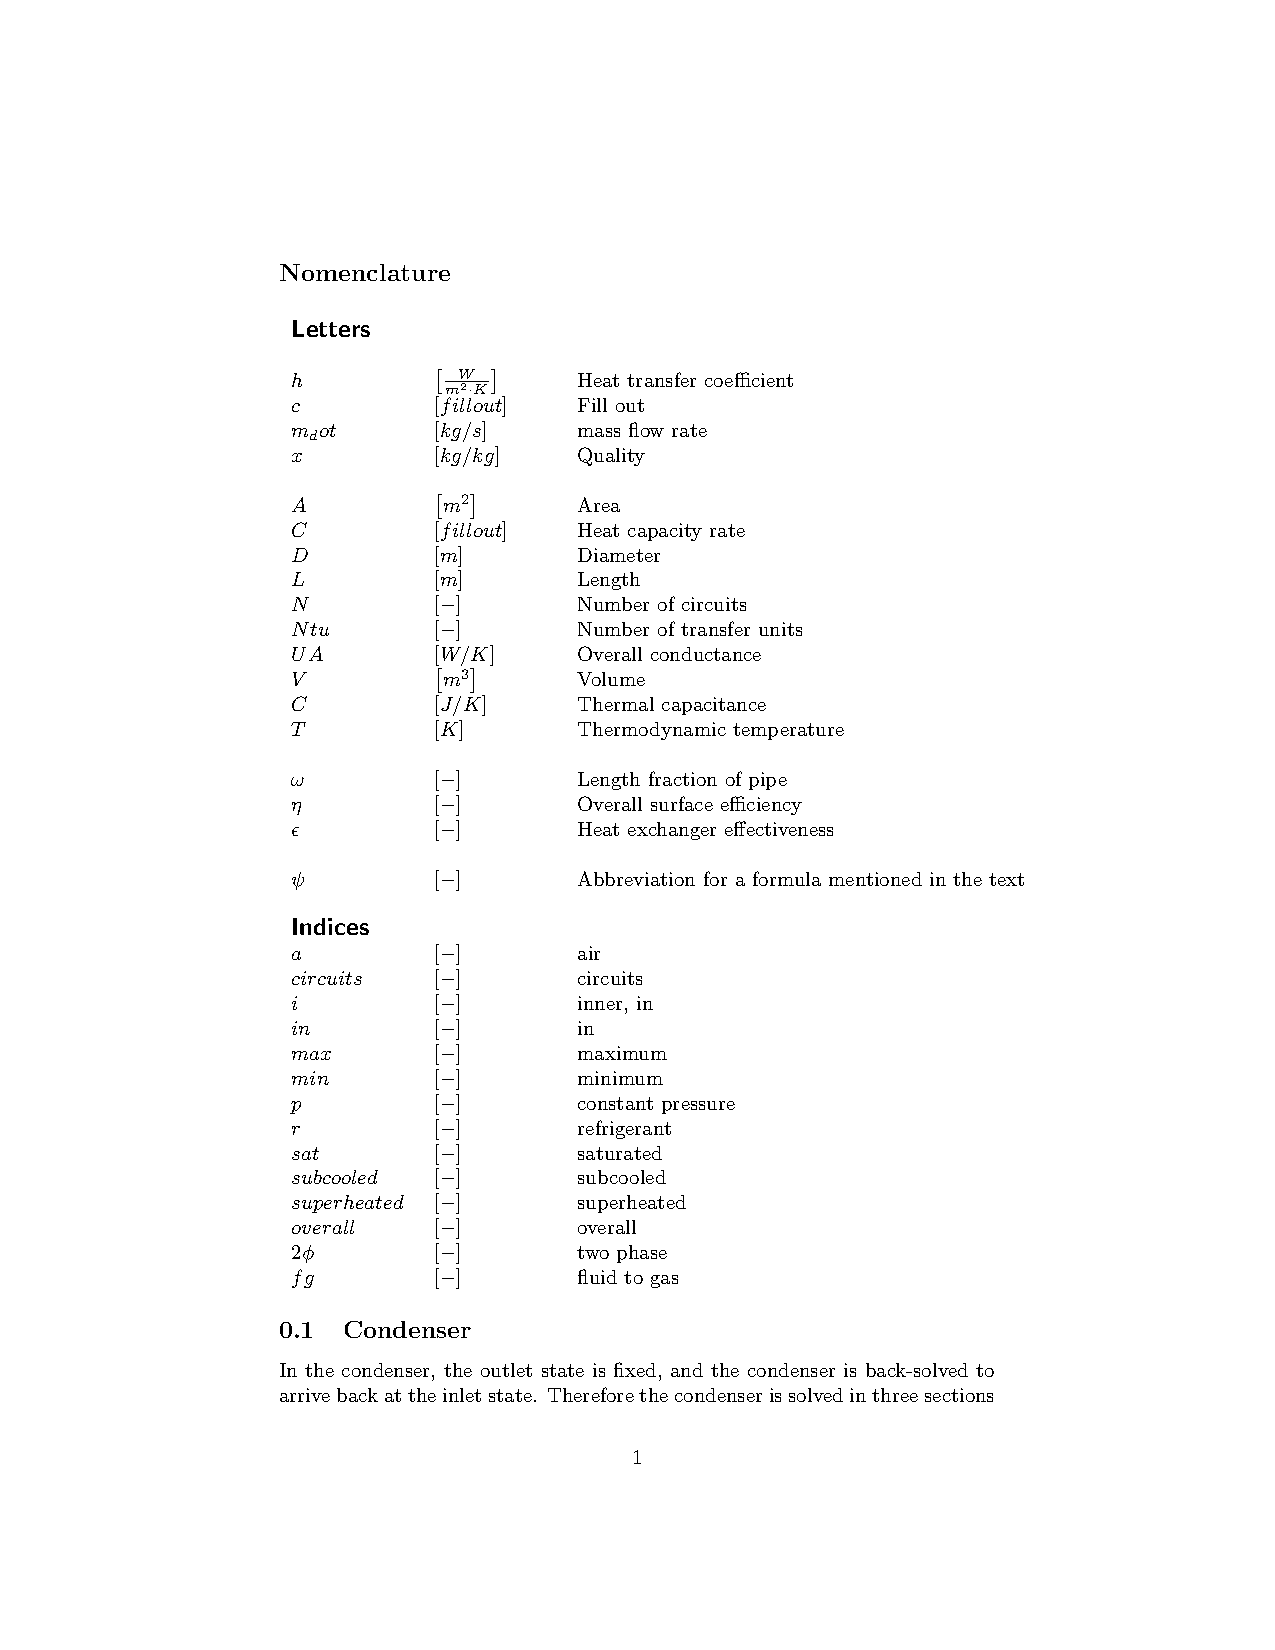
\includegraphics[width=0.8\textwidth]{figs/Condenser}
%\caption{Schematic of condenser}
%\label{fig:Condenser}
%\end{figure}

In the condenser, the outlet state is fixed, and the condenser is back-solved to arrive back at the inlet state.  Therefore the condenser is solved in three sections - the subcooled portion, the two-phase portion, and the superheated portion.  First, the subcooled portion is solved to determine the area fraction required to take the refrigerant at the saturation temperature to the outlet temperature.  Then the fractions of the areas required for the two-phase and superheated sections are found.

The total refrigerant-side volume is equal to
\begin{equation}
V_r=N_{circuits}L_{circuit}\pi \frac{D_i^2}{4}
\end{equation}
The refrigerant-side volume of the three lumps are equal to 
\begin{equation}
\begin{array}{c}
V_{r,subcooled}=w_{subcooled}V_r\\
V_{r,2\phi}=w_{2\phi}V_r\\
V_{r,superheated}=w_{superheated}V_r
\end{array}
\end{equation}

The total refrigerant-side area is equal to
\begin{equation}
A_r=N_{circuits}L_{circuit}\pi D_i
\end{equation} 
and the refrigerant-side areas for each lump are
\begin{equation}
\begin{array}{c}
A_{r,subcooled}=w_{subcooled}A_r\\
A_{r,2\phi}=w_{2\phi}A_r\\
A_{r,superheated}=w_{superheated}A_r
\end{array}
\end{equation}

  \begin{figure*}
  \centerline{
    \mbox{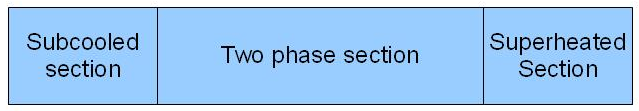
\includegraphics[width=3.00in]{condensorsections.jpg}}
  }
  \caption{Different sections of the condensor - lenght is determined by $w$.}
  \label{overView}
  \end{figure*}


The total air-side area is calculated in the air-side pressure drop and heat transfer correlation routine, and then the air-side area of each of the subcooled, two-phase and superheated regions are equal to the total multiplied by the respective area fraction $w$.

Since the condenser is modeled as pure cross-flow, the air mass flow rate for each section is taken to be equal to the total air mass flow rate multiplied by the respective area fraction $w$.

\subsubsection{Subcooled Section}

\begin{equation}
UA_{subcool} =w_{subcool}\dfrac{1}{  (\eta_a h_a A_{a})^{-1} + (h_{r,subcool} A_{r})^{-1}}\\
\end{equation}
\textbf{If $C_{min}$ on air side:}
\begin{equation}
Ntu_{subcool} = \frac{UA_{subcool}}{w_{subcool}c_{p,a}  \dot m_{a}}
\end{equation}
$w_{subcool}$ cancels out, leaving Ntu independent of $w_{subcool}$.  Energy balance yields
\begin{equation}
\dot m_rc_{p,r}(T_{o,r}-T_{sat,r})=\epsilon_{subcool} C_{min} (T_{i,a}-T_{sat,r})
\end{equation}
\begin{equation}
\dot m_rc_{p,r}(T_{o,r}-T_{sat,r})=\epsilon_{subcool} w_{subcool} c_{p,a}  \dot m_{a} (T_{i,a}-T_{sat,r})
\end{equation}
\begin{equation}
\frac{(T_{o,r}-T_{sat,r})}{(T_{i,a}-T_{sat,r})}=\epsilon_{subcool}C_r
\end{equation}
LHS is constant, call it $\Psi$.  The minimum capacitance rate is on the air side ($C_{min}=  w_{subcool}\dot m_{a,subcool} c_{p,a}$ ), cross-flow with $C_{max}$ mixed (ref.) and $C_{min}$ unmixed (air) yields
\begin{equation}
\epsilon_{subcool} = \displaystyle\frac{1}{C_r} (1 - \exp(-C_r (1 - \exp(-Ntu_{subcool}))))\\
\end{equation}
\begin{equation}
\Psi = (1 - \exp(-C_r (1 - \exp(-Ntu_{subcool}))))\\
\end{equation}
\begin{equation}
\exp(-C_r (1 - \exp(-Ntu_{subcool}))) = 1 - \Psi\\
\end{equation}
\begin{equation}
-C_r (1 - \exp(-Ntu_{subcool})) = \ln(1 - \Psi)\\
\end{equation}
\begin{equation}
C_r  = -\frac{\ln(1 - \Psi)}{(1 - \exp(-Ntu_{subcool}))}\\
\end{equation}

\begin{equation}
w_{subcool}=C_r\frac{\dot m_rc_{p,r}}{\dot m_{a} c_{p,a}}
\end{equation}
\textbf{If $C_{min}$ on refrigerant side:}
\begin{equation}
Ntu_{subcool} = \frac{UA_{subcool}}{\dot m_r c_{p,r}}=\frac{w_{subcool}UA_{overall}}{\dot m_r c_{p,r}}
\end{equation}
\begin{equation}
C_rNtu_{subcool} = \frac{m_r c_{p,r}}{w_{subcool}\dot m_{a,subcool} c_{p,a}}\frac{w_{subcool}UA_{overall}}{\dot m_r c_{p,r}}
\end{equation}
\begin{equation}
C_rNtu_{subcool} = \frac{UA_{overall}}{\dot m_a c_{p,a}}
\end{equation}

Energy balance yields
\begin{equation}
\dot m_rc_{p,r}(T_{o,r}-T_{sat,r})=\epsilon_{subcool} C_{min} (T_{i,a}-T_{sat,r})
\end{equation}
\begin{equation}
\dot m_rc_{p,r}(T_{o,r}-T_{sat,r})=\epsilon_{subcool}\dot m_rc_{p,r} (T_{i,a}-T_{sat,r})
\end{equation}

\begin{equation}
\epsilon_{subcool}=\frac{(T_{o,r}-T_{sat,r})}{(T_{i,a}-T_{sat,r})}
\end{equation}

$C_{min}$ mixed (ref.) and $C_{max}$ unmixed (air) yields
\begin{equation}
\epsilon_{subcool} = 1 - \exp(-\displaystyle\frac{1}{C_r}  (1 - \exp(-C_r Ntu_{subcool})))
\end{equation}
\begin{equation}
\exp(-\displaystyle\frac{1}{C_r}  (1 - \exp(-C_r Ntu_{subcool})))  = 1 - \epsilon_{subcool}
\end{equation}
\begin{equation}
-\dfrac{1}{C_r}  (1 - \exp(-C_r Ntu_{subcool}))  = \log(1 - \epsilon_{subcool})
\end{equation}
\begin{equation}
{C_r}=-\frac{ (1 - \exp(-C_r Ntu_{subcool}))}{\log(1 - \epsilon_{subcool})}=\frac{\dot m_r c_{p,r}}{w_{subcool}\dot m_{a} c_{p,a}}
\end{equation}
\begin{equation}
w_{subcool}=-\frac{\log(1 - \epsilon_{subcool})\dot m_r c_{p,r}}{ (1 - \exp(-C_r Ntu_{subcool}))\dot m_{a} c_{p,a}}
\end{equation}


\subsubsection{Two-Phase}
In the two-phase region, the capacitance rate is only defined for the air-side (yielding a capacitance rate ratio of 0.0), which yields
\begin{equation}
\begin{array}{l}
UA_{2\phi} = w_{2\phi}UA_{overall}\\
Ntu_{2\phi} = \dfrac{UA_{overall} }{c_{p,a}  \dot m_{a}}\\
\epsilon_{2\phi} = 1-\exp(-Ntu_{2\phi})
\end{array}
\end{equation}
Energy balance yields
\begin{equation}
\epsilon_{2\phi}C_{min}(T_{i,a}-T_{sat,r})=\dot m_r h_{fg}
\end{equation}
\begin{equation}
w_{2\phi}=\frac{\dot m_r h_{fg}}{\dot m_a c_{p,a}(T_{i,a}-T_{sat,r})[1-\exp(-Ntu_{2\phi})]}
\end{equation}
Or if there is no superheated section, need to find inlet quality to yield outlet quality of 0.
\begin{equation}
\epsilon_{2\phi}C_{min}(T_{i,a}-T_{sat,r})=-\dot m_r h_{fg}x_{in}
\end{equation}

\begin{equation}
x_{in}\epsilon_{2\phi}=-\frac{\dot m_r h_{fg}}{C_{min}(T_{i,a}-T_{sat,r})}
\end{equation}

The Dekker method varies the area fraction $w_{2\phi}$ which in turn modifies air- and refrigerant-side areas.  Some care must be taken in intermediate iterations to handle the case where the inlet of the condenser is predicted to be in the two-phase region, but in practice the condenser inlet will always be superheated and have a full two-phase region (with the exception of severe under-charge conditions).
	
\subsubsection{Superheated Section}

\begin{equation}
\frac{(T_{sat,r}-T_{in,r})}{(T_{i,a}-T_{in,r})}=\epsilon_{superheat}C_r
\end{equation}
\begin{equation}
 (T_{sat,r}-T_{in,r}) =(T_{i,a}-T_{in,r})\Psi
\end{equation}
\begin{equation}
T_{i,r}=\frac{\Psi T_{i,a}-T_{sat,r}}{\Psi-1}
\end{equation}

In the superheated section, capacitance rate of refrigerant is generally less than that of the air, so the effectiveness can be obtained from
\begin{equation}
\begin{array}{l}
UA_{superheat} = \displaystyle\frac{1}{  (\eta_a h_a A_{a,superheat})^{-1} + (h_{r,superheat} A_{r,superheat})^{-1}}\\[0.6em]
C_r = \displaystyle\frac{c_{p,r}  \dot m_r}{ c_{p,a}  \dot m_{a,superheat}}\\[0.6em]
Ntu_{superheat} = \displaystyle\frac{UA_{superheat}}{c_{p,r}  \dot m_r}\\[0.6em]
\epsilon_{superheat} = 1 - \exp(-\displaystyle\frac{1}{C_r}  (1 - \exp(-C_r Ntu_{superheat})))
\end{array}
\end{equation}
Assuming a constant $c_p$, the condenser refrigerant inlet temperature can be obtained from
\begin{equation}
T_{in,r}=\frac{\Psi T_{i,a}-T_{sat,r}}{\Psi-1}
\end{equation}


\end{document}
